\documentclass[3p,times,procedia]{elsarticle}
\flushbottom
\usepackage{ecrc}
\usepackage{amsmath,amssymb}
\usepackage{booktabs}
\usepackage{graphicx}
\usepackage{float}
\usepackage[bookmarks=false]{hyperref}
\hypersetup{colorlinks,linkcolor=blue,citecolor=blue,urlcolor=blue}
\volume{00}
\firstpage{1}
\journalname{Procedia Computer Science}
\runauth{Madi Gali et al.}
\jid{procs}
\makeatletter
\gdef\@copyrightyear{2026}
\makeatother

\begin{document}
\begin{frontmatter}
\dochead{The 17th International Conference on Emerging Ubiquitous Systems and Pervasive Networks\\
(EUSPN 2026), October 28--30, 2026, Almaty, Kazakhstan}

\title{Evaluating an EMA-Adaptive LSTM for Continuous Behavioral
Authentication on Mobile Devices}

\author[a]{Madi Gali\corref{cor1}}
\author[b]{Vassiliy Serbin}
\author[c]{Aray Kassenkhan}
\address[a]{Department of Cybersecurity, Institute of Automation and
Information Technologies, Satbayev University, Almaty 050013, Kazakhstan}
\address[b]{Department of Information Systems, Institute of Automation and
Information Technologies, Satbayev University, Almaty 050013, Kazakhstan}
\address[c]{Department of Software Engineering, Institute of Automation and
Information Technologies, Satbayev University, Almaty 050013, Kazakhstan}
\cortext[cor1]{Corresponding author.}
\ead{Gali.M@stud.satbayev.university}

\begin{abstract}
Continuous authentication from smartphone inertial sensors must remain useful
when a legitimate user's score distribution changes, yet an adaptive decision
rule can also increase false acceptance or become vulnerable to profile
poisoning. We evaluate a two-layer long short-term memory (LSTM) classifier and
a lightweight agent that updates the first two exponential moving moments of
accepted confidence scores. The study uses accelerometer and gyroscope data
from 100 HMOG subjects. To prevent leakage, the revised protocol reads only the
physical sensor columns, constructs non-overlapping sequences within individual
sessions, keeps complete sessions disjoint between model fitting, validation,
and test, and estimates normalization and initial operating points without test
data. Linear SVM, random forest, and LSTM receive the same 10-second input.
On clean held-out sessions, their macro equal error rates are respectively
$29.92\%\pm0.80\%$, $24.05\%\pm0.86\%$, and
$21.87\%\pm1.01\%$. At the enrollment-derived
operating point, the frozen LSTM threshold and the EMA agent obtain HTERs of
$23.19\%\pm0.95\%$ and $24.53\%\pm1.28\%$ in a balanced alternating
zero-effort attack stress test. Under a standardized synthetic drift of
$\lVert\delta\rVert_2=2$, their HTERs are $24.89\%\pm1.37\%$ and
$26.39\%\pm2.12\%$. Thus the tested EMA rule does not improve the frozen
threshold. These results provide a direct ablation of the adaptive
component and delimit, rather than assume, its benefit. The work's primary
contribution is a reproducible, session-disjoint evaluation of online score
adaptation and an explicit analysis of its security--usability trade-off.
\end{abstract}

\begin{keyword}
continuous authentication \sep behavioral biometrics \sep LSTM \sep
adaptive threshold \sep inertial sensors \sep HMOG \sep concept drift
\end{keyword}
\end{frontmatter}

\section{Introduction}
\label{sec:intro}

One-time authentication cannot protect an unlocked smartphone after control of
the device changes. Continuous authentication (CA) instead evaluates behavioral
signals throughout a session, often without explicit interaction
\cite{alzubaidi_authentication_2016,stylios_behavioral_2021}. Accelerometers and
gyroscopes are attractive for this purpose because they are widely available
and capture user-specific handling and motion patterns
\cite{sitova_hmog_2016,abuhamad_sensorbased_2021}.

The difficulty is temporal change. A classifier trained during enrollment can
become poorly calibrated as posture, task, fatigue, or context changes
\cite{verma_data-driven_2022}. Retraining a deep model after every observation
is impractical on a mobile device, whereas a score-level update is inexpensive.
That convenience is not evidence of effectiveness: an update rule must improve
false rejection without opening the operating point to impostors, and it must
be evaluated causally rather than by selecting a second threshold on test data.

Earlier versions of this study did not isolate that claim. In particular, an
EMA profile was defined but did not participate in the reported decision
equation, LSTM-only ablation and drift experiments were absent, and the data
split was insufficiently documented. The revised study addresses those issues
directly. Its contributions are:

\begin{itemize}
\item a session-disjoint nested protocol in which raw windows and overlapping
contexts cannot cross fit, validation, or test partitions;
\item a decision equation in which the EMA mean and variance determine the
online threshold, with parameters fixed before test evaluation;
\item a controlled LSTM-only versus LSTM+agent ablation at the same initial
operating point, reporting causal FAR, FRR, and HTER decisions; and
\item clean-session and synthetic-drift results with explicit limitations on
external validity and on the interpretation of synthetic covariate shift.
\end{itemize}

\section{Related Work and Scope of Novelty}
\label{sec:related}

CA has a substantial literature. Broad surveys cover system components,
modalities, metrics, privacy, and open deployment problems
\cite{gonzalezmanzano_leveraging_2019,ayeswarya_survey_2019,
stylios_behavioral_2021}. A contemporary smartphone-focused survey catalogs
more than 140 sensor and behavioral-biometric approaches
\cite{abuhamad_sensorbased_2021}. The present work therefore does not claim that
continuous authentication, inertial sensing, LSTM classification, or EMA by
itself is new.

HMOG introduced hand-movement, orientation, and grasp features for smartphone
authentication \cite{sitova_hmog_2016}. Subsequent work applied augmentation,
deep sensor models, and adaptive verification to mobile behavioral data
\cite{li_using_2019,abuhamad_autosen_2020,verma_data-driven_2022}. LSTM and
hybrid recurrent networks are well established for sequential inertial
biometrics \cite{hochreiter_long_1997,zeng_gait-based_2021,giorgi_using_2021}.
Exponentially weighted statistics are likewise standard tools for tracking
non-stationary streams \cite{ross_exponentially_2012,gama_survey_2014}.

\begin{table}[H]
\centering
\small
\caption{Positioning of the present evaluation. A check mark means the cited
work explicitly contains the listed element; protocols and datasets differ, so
reported error rates are not directly comparable.}
\label{tab:position}
\begin{tabular}{lcccc}
\toprule
Work & Inertial & Sequence model & Online update & Drift test \\
\midrule
Sitov\'{a} et al. \cite{sitova_hmog_2016} & $\checkmark$ & -- & -- & -- \\
AUToSen \cite{abuhamad_autosen_2020} & $\checkmark$ & $\checkmark$ & -- & -- \\
Verma et al. \cite{verma_data-driven_2022} & $\checkmark$ & -- & $\checkmark$ & $\checkmark$ \\
This study & $\checkmark$ & $\checkmark$ & $\checkmark$ & $\checkmark$ \\
\bottomrule
\end{tabular}
\end{table}

The narrower novelty is the controlled combination of these elements: a
session-disjoint comparison in which a frozen LSTM threshold and an EMA-updated
threshold start from the same enrollment profile and face the same chronological
test scores. This design isolates adaptation rather than attributing the full
classifier performance to an ``intelligent agent.''

\section{Dataset and Leakage-Resistant Protocol}
\label{sec:data}

\subsection{HMOG data and parsing}

HMOG contains 24 smartphone-interaction sessions for each of 100 participants,
including sitting and walking tasks \cite{sitova_hmog_2016}. We use the
accelerometer and gyroscope. An HMOG inertial CSV row contains metadata before
the three physical axes; consequently, only columns 4--6 are read as $x,y,z$.
This detail is security-critical because a session identifier must never enter
the feature vector. Six empty sensor files belonging to one subject are logged
and skipped; that subject retains enough valid sessions to appear in every
partition.

After a five-second offset, the first 20 non-overlapping windows of 100 samples
are retained from each valid session. Each window is represented by mean,
standard deviation, minimum, maximum, root mean square, and skewness for each of
six channels, producing 36 features. Ten adjacent windows form a 10-second
sequence. The sequence step is also ten windows, so evaluation endpoints do not
share raw samples. Sequences never cross a session boundary.

\subsection{Nested session split}

For session number $r$, define $g(r)=(r-1)\bmod 5$. In outer fold $f$, sessions
with $g(r)=f$ are test sessions, sessions with
$g(r)=(f+1)\bmod 5$ are validation/enrollment sessions, and the remaining
sessions are used to fit the model. Whole sessions, rather than sequences, are
assigned to partitions. Every included subject is required to occur in all
three partitions. This is a session-disjoint cross-validation protocol, not a
claim of leave-one-subject-out or prospective unseen-subject recognition.

A standard scaler is fitted only to the model-fitting sequences and then
applied unchanged to validation and test sequences. Early stopping and initial
threshold estimation use validation data; test labels are not used for either.

\section{Method}
\label{sec:method}

\subsection{System overview}

The system has five stages:

\begin{center}
\fbox{sensor samples} $\rightarrow$
\fbox{1-s windows} $\rightarrow$
\fbox{36 features} $\rightarrow$
\fbox{LSTM score} $\rightarrow$
\fbox{static or EMA decision}
\end{center}

The first four stages are identical in the ablation. Only the last-stage
threshold update changes, which makes any difference in FAR/FRR attributable to
the agent rather than to a different classifier or observation window.

\subsection{LSTM classifier and baselines}

The input is $\mathbf{X}\in\mathbb{R}^{10\times36}$. A two-layer LSTM with 64
hidden units per layer returns its last hidden state. Layer normalization,
a 32-unit ReLU layer, dropout of 0.3, and a 100-class softmax produce claimant
scores $s_{u,n}\in[0,1]$. Training uses cross-entropy, Adam with learning rate
$10^{-3}$, batch size 256, a maximum of 20 epochs, and early-stopping patience 4.

Linear SVM and random forest baselines receive the same sequence flattened to
720 dimensions. The forest contains 300 trees and has minimum leaf size 2.
These baselines compare classifier families at the same temporal endpoint; they
are not presented as adaptive systems.

\subsection{EMA adaptive agent}

For claimant $u$, the validation genuine scores initialize the first and second
moments $p_{u,0}$ and $q_{u,0}$. Before attempt $n$, the agent computes

\begin{align}
\sigma_{u,n-1} &= \sqrt{\max(q_{u,n-1}-p_{u,n-1}^{2},\epsilon^2)},\\
\tau_{u,n} &= \max(0,p_{u,n-1}-k\sigma_{u,n-1}),\\
d_{u,n} &= \mathbb{I}[s_{u,n}\geq\tau_{u,n}].
\end{align}

When $d_{u,n}=1$, the accepted score updates both moments:

\begin{align}
p_{u,n} &= (1-\alpha)p_{u,n-1}+\alpha s_{u,n},\\
q_{u,n} &= (1-\alpha)q_{u,n-1}+\alpha s_{u,n}^{2}.
\end{align}

After a rejection the state is unchanged. Thus repeated unauthenticated events
cannot lower the threshold. An accepted impostor can still poison the profile;
the evaluation deliberately preserves that risk instead of using ground-truth
labels to gate updates.

We fix $\alpha=0.05$, corresponding to an effective memory of approximately
$1/\alpha=20$ accepted attempts. For each claimant, the validation genuine and
impostor scores determine an EER threshold $\tau_{u,0}$; the corresponding
$k_u=(p_{u,0}-\tau_{u,0})/\sigma_{u,0}$ makes the first adaptive threshold
exactly equal to that independently calibrated operating point. Thus $k_u$ is
not selected on test scores. The frozen LSTM ablation uses the same
$\tau_{u,0}$ but never updates it. There is no separate sliding mean and no
unexplained $K=10$ score buffer.

\section{Evaluation}
\label{sec:evaluation}

For each claimant, equal error rate (EER) is found from all exact ROC thresholds
on held-out scores, then macro-averaged across claimants and folds. This EER is a
score-separability statistic; its test-derived crossing threshold is not used
for online decisions.

The static and adaptive decisions are evaluated at their enrollment-derived
operating points. Genuine test attempts follow session and within-session
chronology. Each is alternated with a zero-effort impostor score sampled without
replacement; sampling is repeated ten times. This balanced 50\% attack stream is
an explicit stress test, not an estimate of real attack prevalence. Because the
agent sees no labels, an accepted impostor updates its profile. We report macro
false acceptance rate (FAR), false rejection rate (FRR), and
$\mathrm{HTER}=(\mathrm{FAR}+\mathrm{FRR})/2$.

To isolate score drift, a deterministic direction in standardized 36-feature
space is added progressively over each subject's test chronology. Magnitudes
$\lVert\delta\rVert_2\in\{0,1,2\}$ are tested on the same trained model. This is
a controlled covariate-shift experiment; it does not claim to reproduce every
physiological form of natural behavioral drift.

\section{Results}
\label{sec:results}

\begin{table}[H]
\centering
\caption{Clean held-out-session macro EER (mean $\pm$ standard deviation over
five outer folds). All methods use the same 10-second sequences.}
\label{tab:clean}
\begin{tabular}{lc}
\toprule
Model & EER (\%) \\
\midrule
Linear SVM & $29.92\pm0.80$ \\
Random forest & $24.05\pm0.86$ \\
LSTM (raw score) & $21.87\pm1.01$ \\
\bottomrule
\end{tabular}
\end{table}

Table~\ref{tab:clean} compares score separability. Table~\ref{tab:ablation}
isolates the agent at a threshold estimated without test data. The agent is not
assigned an additional post-hoc EER; its actual causal decisions are reported.

\begin{table}[H]
\centering
\small
\caption{Frozen-threshold and EMA-agent operating points in the balanced
alternating stream (mean $\pm$ standard deviation over five folds).}
\label{tab:ablation}
\begin{tabular}{llccc}
\toprule
$\lVert\delta\rVert_2$ & Decision rule & FAR (\%) & FRR (\%) & HTER (\%) \\
\midrule
0 & Frozen & $22.55\pm1.13$ & $23.82\pm2.27$ & $23.19\pm0.95$ \\
0 & EMA agent & $24.46\pm2.12$ & $24.60\pm2.04$ & $24.53\pm1.28$ \\
1 & Frozen & $22.43\pm0.69$ & $24.82\pm1.97$ & $23.63\pm1.10$ \\
1 & EMA agent & $24.30\pm2.00$ & $25.73\pm2.64$ & $25.02\pm1.66$ \\
2 & Frozen & $22.40\pm0.85$ & $27.37\pm2.91$ & $24.89\pm1.37$ \\
2 & EMA agent & $24.53\pm2.11$ & $28.25\pm4.25$ & $26.39\pm2.12$ \\
\bottomrule
\end{tabular}
\end{table}

\begin{figure}[H]
\centering
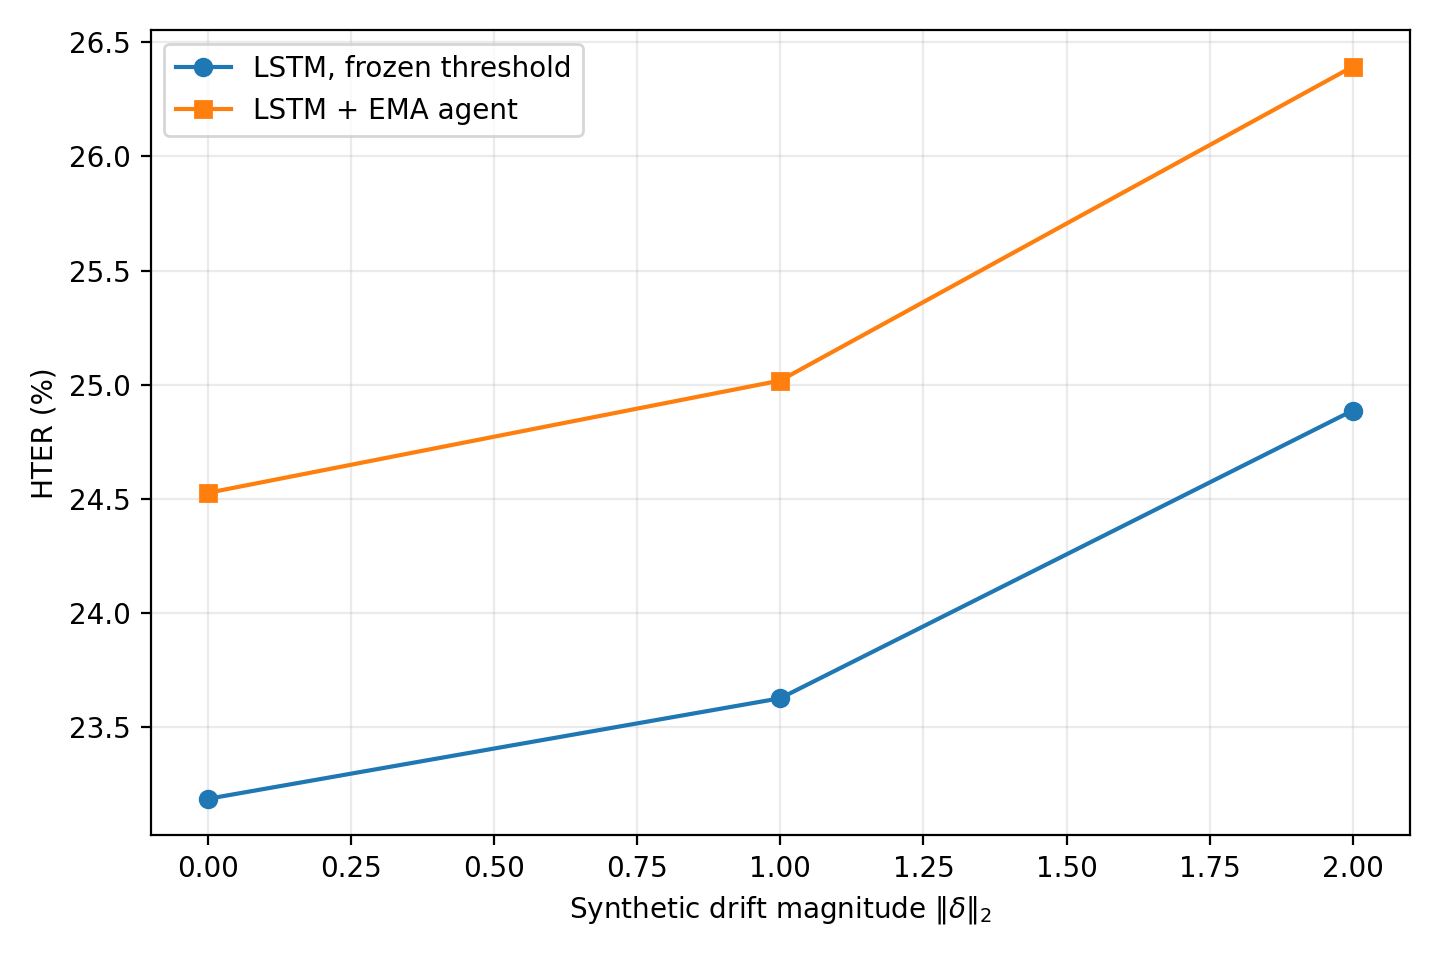
\includegraphics[width=0.82\columnwidth]{revised_results/revised_drift_hter.png}
\caption{HTER of the frozen LSTM threshold and EMA agent under synthetic
standardized-feature drift. Error bars are omitted because fold-level values
are reported in the accompanying result file.}
\label{fig:drift}
\end{figure}

On clean data, the LSTM lowers macro EER by 2.18 percentage points relative to
RF and by 8.05 points relative to the linear SVM. These values are much higher
than the invalid figures produced when metadata columns entered the feature
vector, illustrating why the leakage correction is substantive.

The agent ablation is negative. On clean sessions, adaptation increases HTER by
1.34 points. At drift magnitudes 1 and 2, it increases HTER by 1.39 and 1.51
points, respectively. The frozen threshold has lower HTER in every one of the
five folds at all three drift levels. Adaptation increases both FAR and FRR on
average; therefore its poorer HTER cannot be characterized as a deliberate
security--usability trade. Both decision rules degrade as drift grows, and the
tested EMA mechanism does not preserve the operating point better than the
static comparator.

\section{Discussion}
\label{sec:discussion}

The revised experiment separates three questions that were previously mixed.
First, Table~\ref{tab:clean} measures whether the LSTM score distinguishes a
claimant from zero-effort impostors. Second, Table~\ref{tab:ablation} measures
whether an independently initialized operating point is usable without
recalibration. Third, Fig.~\ref{fig:drift} asks whether EMA adaptation changes
that operating point under a controlled shift. A low EER alone does not prove
that the agent contributes, and a lower FRR is not a benefit if FAR rises enough
to worsen HTER.

The accepted-only update is intentionally lightweight and causal. It avoids the
clearly unsafe behavior of lowering a threshold after rejection, but it cannot
adapt to scores that fall below the current threshold. It also remains exposed
to poisoning after false acceptance. A deployable design should combine
high-confidence update gates, step-up authentication, and explicit poisoning
tests.

\subsection{Limitations}

Only HMOG is evaluated. This directly limits external validity and does not
satisfy the stronger claim that the method generalizes across devices,
populations, or sensor corpora. A second session-rich dataset is required before
making such a claim. Six empty sessions are skipped and documented. The
modulo-session split prevents sample overlap but is not a rolling-origin
forecast of a newly enrolled user. The alternating 50\% impostor stream is a
security stress test rather than a real-world prevalence model. The synthetic
drift is defined in feature space and uses one direction per fold; future work
should include multiple directions, sensor bias/scale/rotation perturbations,
natural late-session drift, confidence intervals clustered by session, and
live on-device latency and energy measurements.

Comparisons with published numbers are intentionally not ranked. Prior studies
use different activities, modalities, enrollment sizes, subject sets, and split
rules, so claiming superiority from EER alone would be misleading.

\section{Conclusion}

This work presents a reproducible evaluation of an LSTM with an EMA-updated
authentication threshold on HMOG. The revised pipeline removes identifier
leakage, uses complete session-disjoint partitions, separates validation from
training, provides the missing LSTM-only ablation, and tests the adaptive
mechanism under controlled drift. The LSTM has the best clean EER among the
three classifiers, but the EMA agent consistently worsens HTER relative to the
same LSTM with a frozen threshold. The tested agent should therefore not be
deployed or presented as a successful drift solution. The evidence supports only
the measured HMOG protocol; broader effectiveness requires independent-dataset
and live-stream validation.

\section*{Reproducibility Statement}

The companion code records sensor-column selection, fold assignments, skipped
sessions, random seed, hyperparameters, per-fold results, and aggregate
summaries. The canonical entry point is \texttt{hmog\_revised\_experiment.py};
legacy result files are excluded from the revised manuscript.

\bibliographystyle{elsarticle-num}
\bibliography{references}
\end{document}
